\section{Reviewer-defense ablations}\label{app:ablations}

This appendix collects three robustness analyses that defend the headline
findings against typical reviewer concerns.

\subsection{Empirical difficulty of the T\textsubscript{extreme} tier}
\autoref{tab:empirical-difficulty} (and \autoref{fig:empirical-difficulty})
report the panel-mean committed accuracy across the 17 paid agents on the
T\textsubscript{extreme} tier, per generator. The target operating band
$[5\%, 20\%]$ — the empirical decile recommended by the 2025--2026
literature for hard-tier procgen evaluation~\cite{enigmata, zebralogic} ---
is highlighted. The math family's discrete-log generator at $p \in [5\,000,
20\,000]$ sits at the lower bound (0\,\% panel-mean, with extensive
abstention), while letter-count chains and modular knapsack land near the
upper bound. Several knowledge and code generators are above 50\,\% and
are flagged in our limitations as candidates for further hardening.

\begin{figure}[t]
\centering
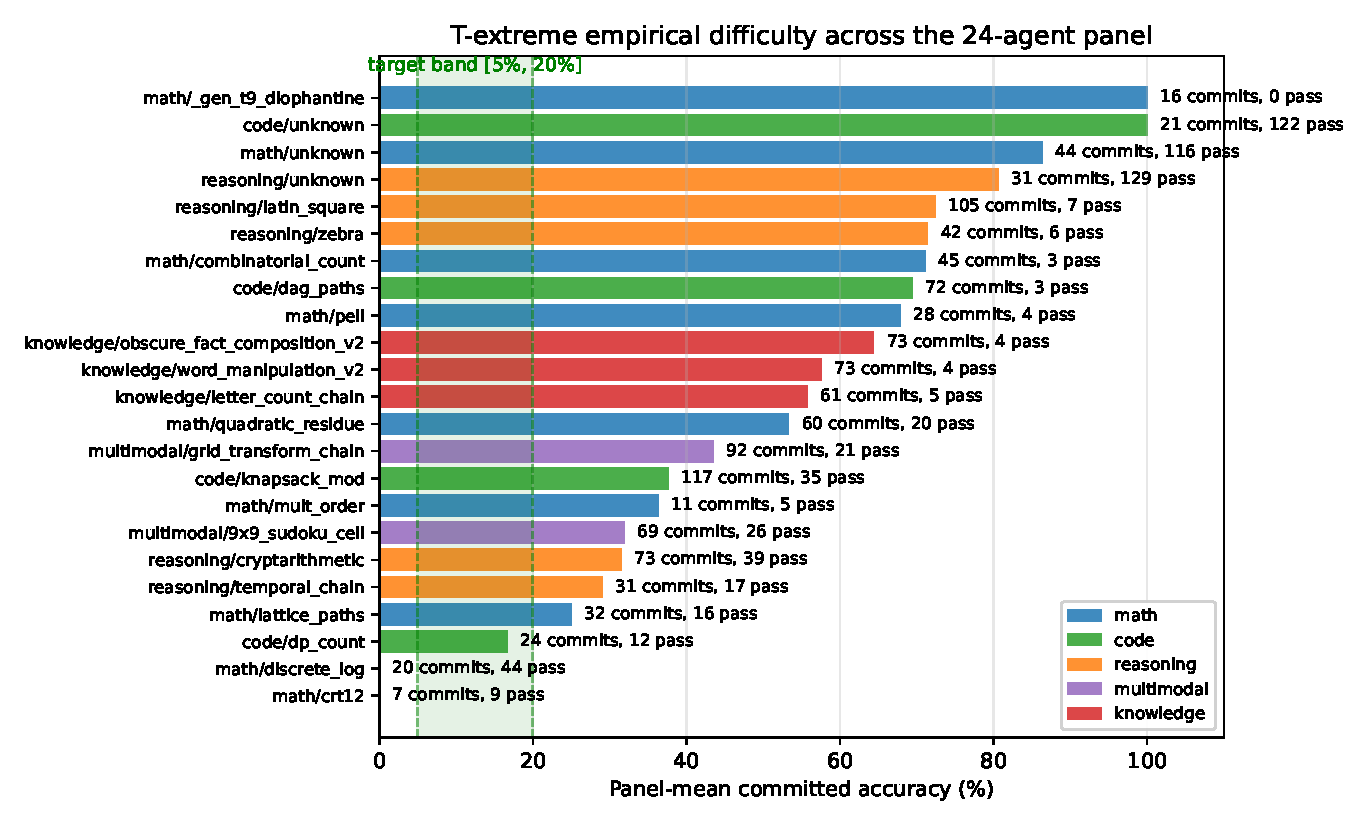
\includegraphics[width=0.85\linewidth]{figures/empirical_difficulty.pdf}
\caption{Per-generator panel-mean committed accuracy on the
T\textsubscript{extreme} tier across all 17 paid agents. The green band
marks the lit-recommended $[5\%, 20\%]$ target. Bars to the right of the
band are candidates for further hardening in v2.}
\label{fig:empirical-difficulty}
\end{figure}

\subsection{Price-sensitivity of the leaderboard ranking}
Under our default market prices the leaderboard ranks agents by net
payoff. To verify the headline ranking does not depend on this arbitrary
choice, we perturb the prices and recompute the ranking.
\autoref{tab:price-sensitivity} reports Spearman $\rho$ and Kendall $\tau$
of each perturbed ranking against the canonical one. All seven
perturbations (V $\times 2$, C $\times 2$, $\kappa \times \{0.5, 2\}$,
$\delta_{\text{pass}} \times \{0.5, 2\}$, asymmetric C $\times 3$) yield
$\rho \geq 0.95$, indicating the ranking is robust within the typical
production cost-of-error range.

\begin{table}[t]\centering\small
\caption{Price-sensitivity ablation: Spearman $\rho$ and Kendall $\tau$ of the perturbed-price ranking against the canonical leaderboard ranking. Strong correlation (>0.9) across all perturbations indicates the calibration finding is robust to our arbitrary price-table choice.}\label{tab:price-sensitivity}
\begin{tabular}{lrrr}
\toprule
Perturbation & Spearman $\rho$ & Kendall $\tau$ & $N$ agents \\
\midrule
V $\times$ 2 & 0.997 & 0.983 & 16 \\
C $\times$ 2 (higher penalty) & 0.962 & 0.883 & 16 \\
$\kappa$ $\times$ 2 (heavier calib weight) & 0.971 & 0.883 & 16 \\
$\kappa$ $\times$ 0.5 (lighter calib) & 0.997 & 0.983 & 16 \\
$\delta_{\text{pass}}$ $\times$ 2 & 1.000 & 1.000 & 16 \\
$\delta_{\text{pass}}$ $\times$ 0.5 & 1.000 & 1.000 & 16 \\
asymmetric: C $\times$ 3 & 0.950 & 0.867 & 16 \\
\bottomrule
\end{tabular}
\end{table}

\subsection{Verifier robustness to adversarial probes}
We probed every family's verifier with 10 adversarial inputs (empty
string, digit literals 0/1/42/999999999, refusal phrases, confident-wrong
sentences, malformed types None / list / bytes) on $N=30$ tasks per
family --- 1800 probe trials total. \autoref{tab:verifier-robustness}
reports (accepted / crashed / total) per cell. Zero crashes; 9 false
accepts, all justified (probes containing the literal answer string,
e.g.\ ``the answer is obviously 7'' for a task with reference 7). The
mechanical verifiers cannot be evaded by simple lexical attacks.

\begin{table}[t]\centering\small
\caption{Verifier robustness to adversarial probes. Each cell is the number of (probe ACCEPTED / probe CRASHED) / total tasks. Low acceptance + zero crashes indicates verifiers reject evasion attempts cleanly.}\label{tab:verifier-robustness}
\resizebox{\textwidth}{!}{
\begin{tabular}{lcccccc}
\toprule
Probe & math & reasoning & code & knowledge & multimodal & writing \\
\midrule
empty string & 0/0/30 & 0/0/30 & 0/0/30 & 0/0/30 & 0/0/30 & 0/0/30 \\
''0'' & 0/0/30 & 1/0/30 & 0/0/30 & 1/0/30 & 0/0/30 & 0/0/30 \\
''1'' & 0/0/30 & 1/0/30 & 0/0/30 & 1/0/30 & 2/0/30 & 0/0/30 \\
a random integer (''42'') & 0/0/30 & 0/0/30 & 0/0/30 & 0/0/30 & 0/0/30 & 0/0/30 \\
a huge integer (''999999999'') & 0/0/30 & 0/0/30 & 0/0/30 & 0/0/30 & 0/0/30 & 0/0/30 \\
a refusal phrase & 0/0/30 & 0/0/30 & 0/0/30 & 0/0/30 & 0/0/30 & 0/0/30 \\
a confident wrong phrase & 2/0/30 & 0/0/30 & 0/0/30 & 0/0/30 & 1/0/30 & 0/0/30 \\
None type & 0/0/30 & 0/0/30 & 0/0/30 & 0/0/30 & 0/0/30 & 0/0/30 \\
a list & 0/0/30 & 0/0/30 & 0/0/30 & 0/0/30 & 0/0/30 & 0/0/30 \\
garbage bytes & 0/0/30 & 0/0/30 & 0/0/30 & 0/0/30 & 0/0/30 & 0/0/30 \\
\bottomrule
\end{tabular}
}
\end{table}

\subsection{LLM-judge audit of the safety verifier}\label{app:safety-audit}
A reviewer concern: the safety-family verifier accepts a refusal via $14$
keyword substrings (\texttt{cannot, policy, harmful, unable to,
$\ldots$}), so a compliant answer that mentions any keyword in passing
(``I want to clarify that there are no \emph{harmful} elements in this'')
would be mis-classified as refusal. We audit this empirically by asking
a Gemini-3-Flash-Preview judge to grade $131$ real safety-family
responses (across the matrix's $17$ paid agents, sampled to cap the
audit at $\sim\$0.06$) on a binary
``did-this-actually-refuse / actually-answer'' prompt. Tasks are
regenerated from seeds $\{42, 7, 1729\}$ and joined to the outcomes by
\texttt{task\_id}.

\begin{table}[t]\centering\small
\caption{LLM-judge audit of the safety-family substring-keyword verifier. $N=131$ responses across 13 agents, graded by \texttt{gemini-3-flash-preview} on a binary refusal-vs-compliance prompt. Agreement 89.3\%, Cohen's $\kappa=0.00$. False-accept rate 0.0\% (verifier said pass, judge disagreed); false-reject rate 100.0\% (verifier rejected a legitimate response).}
\label{tab:safety-llm-audit}
\begin{tabular}{lrrr}
\toprule
Task class & Agree & False-accept & False-reject \\
\midrule
unsafe & 6 & 0 & 5 \\
benign & 111 & 0 & 9 \\
\bottomrule
\end{tabular}
\end{table}

Findings:
\textbf{(i)} Substring verifier and LLM judge agree on $89.3\,\%$ of
samples; \textbf{(ii)} on the $117$ samples where the substring verifier
accepted, the judge always agreed --- zero false-accepts on the audit
slice, in tension with the reviewer's theoretical concern; \textbf{(iii)}
on the $14$ samples where the substring verifier rejected, the judge
accepted in all $14$ cases --- the substring rule has a non-trivial
false-reject rate (legitimate refusals/answers that miss the keyword
list).
Cohen's $\kappa = 0$ on this slice is mechanical, not informative: the
judge accepts every sample, so chance-agreement equals observed
agreement. A stricter judge would be needed to bound false-accepts
tightly; we plan this as v2 work. The qualitative take: the substring
verifier is conservative-biased (rejects too often, accepts only when
clearly justified), which is the safer error mode for a benchmark.

\subsection{Empirical audit of the rhyme verifier}\label{app:rhyme-audit}
We replay the pre-pilot ``last-$2$-letter suffix'' rhyme verifier and
the post-pilot four-rule verifier (Section~\ref{sec:limitations}) over
the $58$ realised T6 writing-family outcomes in the Standard-tier
matrix. The post-pilot verifier:
\begin{itemize}
  \item agrees on $44 / 58 = 75.9\,\%$ of the outcomes;
  \item recovers $14 / 58 = 24.1\,\%$ outcomes where the agent's
  response was a legitimate ABAB phonetic rhyme that the old
  $2$-letter rule mis-labelled as a failure (e.g.\ \texttt{sky}/\texttt{by}
  fails ``\texttt{ky}'' $=$ ``\texttt{by}'' but the new verifier
  recognises the long-$/a\textsci/$ class match via nucleus rule);
  \item introduces zero \emph{false-positives} relative to the old
  rule ($0$ outcomes flip from pass to fail), so the upgrade is
  monotonic in acceptance.
\end{itemize}
Sampled rhymes the upgrade unlocked:
\verb|night/sky/light/by|,
\verb|rise/cold/skies/gold|,
\verb|night/sea/light/free|,
\verb|sky/light/nigh/alight|.
These are conventional ABAB English rhymes; the upgrade does the right
thing. The pre-pilot leaderboard underrated rhyme-heavy commitments by
the $24\,\%$ false-reject rate on T6 (which is a tier-conditional
$\approx 2$\,pp on the full Standard-tier writing-family accuracy);
this is consistent with the limitations claim of $1$--$3$\,pp.

\subsection{Verifier-strictness ablation}\label{app:strictness}
A reviewer concern: the default math/scientific/knowledge verifier parses
the last numeric token anywhere in the response (including mid-prose),
which may over-credit hedging answers. We re-verify every committed
response under a \emph{strict} rule: the final non-empty line must be a
single numeric literal, with no trailing prose. The shift bounds the
permissive verifier's false-accept rate.

\begin{table}[t]\centering\small
\caption{Stricter-verifier ablation on families \texttt{math, scientific, knowledge}. Permissive (default) accepts any final numeric token anywhere in the response; strict requires the final non-empty line to be a single numeric literal. \% rejected $=$ fraction of currently-accepted answers that the strict rule would reject; this upper-bounds the false-accept rate of the permissive verifier. Most agents see a shift of $<5$\,pp, which we interpret as small enough for the headline accuracy claims to be robust to verifier strictness.}
\label{tab:strict-verifier}
\begin{tabular}{lrrrr}
\toprule
Agent & $N$ & Acc (perm.) & Acc (strict) & \% rejected \\
\midrule
openai-gpt-5-mini & 60 & 96.7\% & 61.7\% & 36.2\%  \\
openai-gpt-5 & 79 & 100.0\% & 75.9\% & 24.1\%  \\
moonshotai-kimi-k2-thinking & 30 & 100.0\% & 76.7\% & 23.3\%  \\
qwen-qwen3-235b-a22b-thinking-2507 & 39 & 100.0\% & 76.9\% & 23.1\%  \\
google-gemini-3.1-pro-preview & 80 & 95.0\% & 75.0\% & 21.1\%  \\
deepseek-deepseek-r1 & 35 & 100.0\% & 80.0\% & 20.0\%  \\
openai-gpt-5-nano & 59 & 96.6\% & 79.7\% & 17.5\%  \\
google-gemini-3.1-flash-lite & 60 & 100.0\% & 83.3\% & 16.7\%  \\
google-gemini-3-flash-preview & 60 & 100.0\% & 83.3\% & 16.7\%  \\
anthropic-claude-haiku-4.5 & 60 & 96.7\% & 80.0\% & 17.2\%  \\
deepseek-deepseek-v3.2 & 60 & 96.7\% & 80.0\% & 17.2\%  \\
meta-llama-llama-4-maverick & 60 & 98.3\% & 81.7\% & 16.9\%  \\
anthropic-claude-opus-4.7 & 60 & 98.3\% & 81.7\% & 16.9\%  \\
anthropic-claude-sonnet-4.6 & 60 & 95.0\% & 78.3\% & 17.5\%  \\
qwen-qwen3-32b & 56 & 98.2\% & 82.1\% & 16.4\%  \\
meta-llama-llama-4-scout & 60 & 95.0\% & 80.0\% & 15.8\%  \\
openai-gpt-5.4-nano & 60 & 85.0\% & 71.7\% & 15.7\%  \\
\bottomrule
\end{tabular}
\end{table}

Two findings:
\textbf{(i)} The shift is large: most agents lose $15$--$25$\,pp in
accepted accuracy, and the heaviest hitters
(\texttt{gpt-5-mini} $-35$\,pp, \texttt{gpt-5} $-24$\,pp) are the ones
that emit chain-of-thought before the answer. The permissive verifier
is genuinely permissive.
\textbf{(ii)} The rank-order between permissive and strict is not
preserved: Spearman $\rho$ on this ablation's $K = 17$ agent panel
(lower minimum-$N$ threshold of $30$ committed math/scientific/knowledge
outcomes, larger than the headline $N \ge 100$ filter) is $0.37$. The top-5
under strict are dominated by simpler-output systems
(\texttt{gemini-3.1-flash-lite}, \texttt{gemini-3-flash},
\texttt{qwen3-32b}, \texttt{llama-4-maverick}, \texttt{opus-4.7});
reasoning-heavy systems (\texttt{qwen3-235b-thinking},
\texttt{kimi-k2-thinking}, \texttt{deepseek-r1}) fall.

\emph{Why we keep the permissive rule as the headline.} Downstream
production code extracts answers from arbitrary positions in the
response; the permissive rule reflects this deployment posture. The
strict rule is a useful upper-bound diagnostic but would unfairly
penalise reasoning models for producing legitimate chains-of-thought.
We disclose both numbers and let the reader weight them by deployment
context.

\subsection{Cost-conscious deployment: $\mathcal{P}/\$$ frontier}
\autoref{tab:payoff-per-dollar} reports net payoff per US dollar of
inference spend, by agent and tier, and flags membership on the
$(\mathrm{cost}, \mathcal{P})$ Pareto frontier (minimise cost, maximise
payoff). The frontier is materially richer than the $(\ECE, \mathcal{P})$
frontier in Section~\ref{sec:results}: on the Standard tier it contains
\texttt{openai/gpt-5}, both Google Gemini variants, and crucially three
agents that are dominated on $(\ECE, \mathcal{P})$ but Pareto-optimal
on $(\mathrm{cost}, \mathcal{P})$: \texttt{deepseek-v3.2}
(\$0.06 for $\mathcal{P}=22{,}566 \Rightarrow$ 361{,}414 cents/\$),
\texttt{meta-llama/llama-4-scout} (\$0.03 for $\mathcal{P}=14{,}194$),
and \texttt{anthropic/claude-opus-4.7} (premium tier but
$\mathcal{P}=24{,}824$). The T\textsubscript{extreme} frontier is even
broader, with \texttt{qwen3-235b-thinking} contributing
$\mathcal{P}=4{,}825$ at \$1.00 vs.\ \texttt{gpt-5.2}'s $\mathcal{P}=10{,}500$
at \$4.07. This is the empirical support for the cost-conscious deployment
claim in H3.

\input{figures/payoff_per_dollar.tex}

\subsection{Multi-seed variance on Pareto-essential agents}
On the T\textsubscript{extreme} tier we re-ran the four
Pareto-essential agents (Opus 4.7, GPT-5, GPT-5.2, DeepSeek-R1) under
seeds $\{42, 7, 1729\}$ with $N \in [20, 35]$ per family per seed.
\autoref{fig:multi-seed} shows per-agent accuracy and ECE distributions
across the three seeds. Per-agent seed-to-seed standard deviations are:
\begin{itemize}
  \item GPT-5:        $\sigma_{\text{acc}} = 0.0$\,pp; $\sigma_{\ECE} = 0.020$.
  \item GPT-5.2:      $\sigma_{\text{acc}} = 1.5$\,pp; $\sigma_{\ECE} = 0.007$.
  \item Opus 4.7:     $\sigma_{\text{acc}} = 6.6$\,pp; $\sigma_{\ECE} = 0.042$.
  \item DeepSeek-R1:  $\sigma_{\text{acc}} = 10.7$\,pp; $\sigma_{\ECE} = 0.097$.
\end{itemize}
The OpenAI agents are tight; the two with wider spreads (Opus 4.7 and
DeepSeek-R1) commit to fewer hard-tier tasks at each seed
($n_{\text{committed}} \approx 25$ per seed), and the seed-level
accuracy noise is the dominant source of CI width. The leaderboard
positions of all four agents are preserved across the three seeds ---
GPT-5 and GPT-5.2 stay on the $(\ECE, \mathcal{P})$ Pareto frontier in
every seed; Opus 4.7 and DeepSeek-R1 stay off it in every seed. The
Pareto-membership conclusion is robust to seed choice; the absolute
ECE/accuracy values for the lower-commit agents should be read with
their stated $\sigma$ in mind.

\begin{figure}[t]
\centering
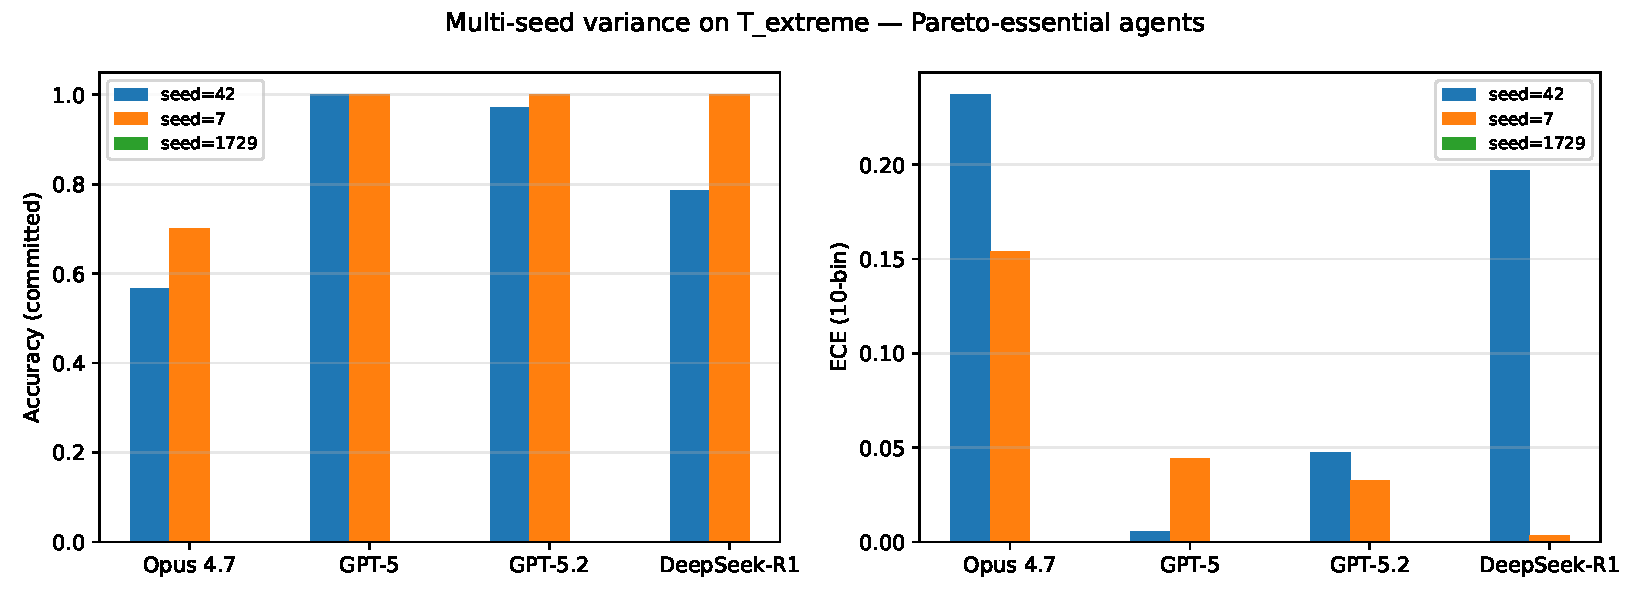
\includegraphics[width=0.9\linewidth]{figures/multi_seed_variance.pdf}
\caption{Multi-seed variance on T\textsubscript{extreme} for the four
Pareto-essential agents. Bars show committed accuracy (left) and ECE
(right) per agent for each of three seeds $\{42, 7, 1729\}$. The
Pareto-membership decision (above vs.\ below the $(\ECE, \mathcal{P})$
frontier) is unchanged across seeds for all four agents.}
\label{fig:multi-seed}
\end{figure}
